\chapter{Результаты расчетов для выборки по варианту}

%\begin{figure}[H]
%	\centering
%	\begin{tabular}{|c|c|}
%		\hline
%		$M_{min}$ & -12.2\\
%		\hline
%		$M_{max}$ & -7.77\\
%		\hline
%		$R$ & 4.43\\
%		\hline
%		$\hat \mu (\vec x_n)$ & -10.1318\\
%		\hline
%		$S^2(\vec x_n)$ & 0.846041\\
%		\hline
%		$m$ & 8\\
%		\hline
%	\end{tabular}
%\end{figure}

\begin{figure}[H]
	\centering
	\begin{tabular}{|c|c|c|c|c|c|}
		\hline
		$M_{min}$ & $M_{max}$ & $R$ & $\hat \mu (\vec x_n)$ & $S^2(\vec x_n)$ & $m$\\
		\hline
		-12.2 & -7.77 & 4.43 & -10.1318 & 0.846041 & 8\\
		\hline
	\end{tabular}
\end{figure}

\begin{figure}[H]
	\centering
	\begin{tabular}{|c|c|c|}
		\hline
		$i$ & $J_i$ & $n_i$\\
		\hline
		1 & $[-12.20; -11.65)$ & 4\\
		\hline
		2 & $[-11.65; -11.09)$ & 15\\
		\hline
		3 & $[-11.09; -10.54)$ & 23\\
		\hline
		4 & $[-10.54;  -9.98)$ & 27\\
		\hline
		5 & $[ -9.98;  -9.43)$ & 17\\
		\hline
		6 & $[ -9.43;  -8.88)$ & 25\\
		\hline 
		7 & $[ -8.88;  -8.32)$  & 6\\
		\hline
		8 &  $[ -8.32;  -7.77]$ & 3\\
		\hline
	\end{tabular}
\end{figure}

\begin{figure}[H]
	\begin{center}
		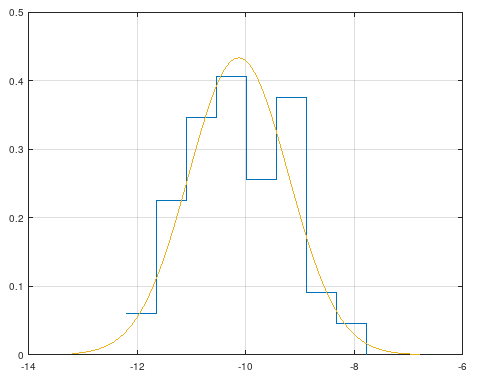
\includegraphics[scale=0.78]{assets/fst.png}
	\end{center}
	\caption{Гистограмма и график функции плотности распределения вероятностей нормальной случайной величины с выборочными мат. ожиданием и дисперсией}
\end{figure}

\begin{figure}[H]
	\begin{center}
		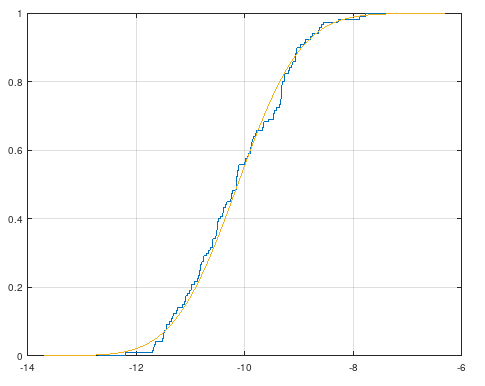
\includegraphics[scale=0.78]{assets/scnd.png}
	\end{center}
	\caption{График эмпирической функции распределения и функции распределения нормаль-
		ной случайной величины с выборочными мат. ожиданием и дисперсией}
\end{figure}